\begin{figure}
\centering
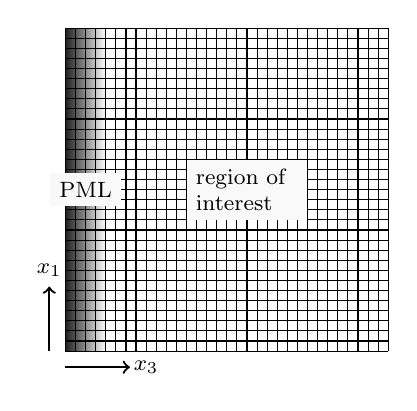
\begin{tikzpicture}[scale=4.1]
\tikzstyle{every node}=[font=\footnotesize]

\draw[->,thick] (-0.05,0) -- (-0.05,0.2);
\draw (-0.05,0.25) node {$x_1$};

\draw[->,thick] (0,-0.05) -- (0.2,-0.05);
\draw (0.25,-0.05) node {$x_3$};

% Fill in the PML region 
\shade[left color=black!87!,inner color=gray,right color=white]
  (0,0) rectangle (0.125,1);

% Main box, (0,1) x (0,1)
\draw[step=0.03125] (0,0) grid (1,1);

\node[fill=gray!5!,text width=1.3cm] (note1) at (0.5625,0.5)
{region of interest};

\draw (0.0625,0.5   ) node[fill=gray!5!] {PML};

\end{tikzpicture}
\caption{An $x_1 x_3$ cross section of a cube with PML on its $x_3=0$ face.
The domain is shaded in a manner which loosely corresponds to its extension into
the complex plane.}
\label{fig:plane-with-single-pml}
\end{figure}
